% !TeX spellcheck = en_US
\chapter{Robotics Foundations}

\section{Introduction}
Types of robots:
\begin{center}
	\begin{tabular}{m{2cm}|m{2.2cm}|m{1.5cm}|m{2.7cm}|m{2.2cm}|m{2cm}}
		Types & Articulated robot & Gantry & Scara & Delta & Hexapod\\ \hline\hline
		Workspace & Large & & & Small & Small \\\hline
		Structure & 6 rotational & 3 linear & 1 translational, 2-3 parallel rotational & 3 parallel kinematics chains & 6 parallel kinematics chains\\ \hline
		Market share & 68\% & 19\% & 11\% & 1\%	& 1\%
	\end{tabular}
\end{center}

\section{DH Convention}
\ac{DH} Convention: \todo{}

Elementary rotation matrices:
\begin{figure}[hbt!]
	\centering
	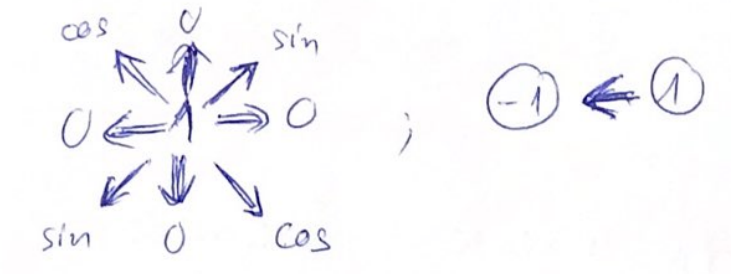
\includegraphics[width=0.5\textwidth]{elementary-rotation-matrix.png}
\end{figure}

\section{Position \& Orientation}
\begin{itemize}
	\item Euler angles: \textbf{12} different sets of angles $R_{xy'z''}(\Phi) = R_z(\varphi) R_{y'}(\theta) R_{z''}(\psi)$
	\item Roll-Pitch-Yaw: fixed frame $XYZ$ $R(\varphi, \theta, \psi) = R_z(\varphi) R_y(\theta) R_x(\psi)$
	\item Gimbal lock: loss of 1 \ac{dof} in a 3-dimensional, 3 gimbal mechanism when 2/3 gimbals are driven into a parallel configuration\\
	\note It exists no matter what rotation sequence you choose
	\item Angle \& axix representation: solves gimbal lock problem\\
	However, does not guarantee an unique solution. When doing inverse, has problem when $\sin \theta=0$
	\item Unit quaternion: \hlb{CAN} describe any rotation without ambiguities!
\end{itemize}
\hlb{Intuition:} angle \& axis representation, unit quaternion are ways to avoid dealing with/or deal better with gimbal lock

\section{Actuators and Joints}
\section{Workspace}

\section{Kinematics}
\subsection{Direct Kinematics}
\begin{itemize}
	\item Homogeneous coordinate representation, transformation matrix
	\item $\vec{e}_{x, \prescript{i}{}{o}} = \vec{e}_{z, \prescript{i-1}{}{o}} \times \vec{e}_{z, \prescript{i}{}{o}}$
\end{itemize}

\subsection{Inverse Kinematics}
\begin{itemize}
	\item Kinematic redundancy: No $\rightarrow$ Functional $\rightarrow$ hyper
	\item 3 ways to solve:
	\begin{itemize}
		\item Analytical: if analytical solution exists, \hlb{ALWAYS} use it. Non redundant
		\item Numerical: If closed-form solution does not exist / too hard to find analytically. If redundant
		\begin{align*}
			err &= r_d - f(q_e)\\
			q_{k+1} &= q_k + \frac{1}{J_A(q)} adj(J_A(q)) err_k
		\end{align*}
		\item Algebraic: solve polynomials equations
	\end{itemize}
\end{itemize}

\subsection{Differential Kinematics}
{\color{red} \boxed{\text{joint velocity $\Rightarrow$ \ac{ee} velocity}}}

\hlb{Using Geometric Jacobian}
\begin{align}
	&q = [q_1 \dots q_n]^T &&-\text{joint positions}\\
	&v_E = \begin{bmatrix}
		\dot{p}_E\\
		\omega_E
	\end{bmatrix} &&-\text{\ac{ee} velocity}\\
	&\dot{p}_E = [\dot{p}_x \quad \dot{p}_y \quad \dot{p}_z]^T &&-\text{\ac{ee} linear velocity}\\
	&\omega_E = [\omega_x \quad \omega_y \quad \omega_z]^T &&-\text{\ac{ee} angular velocity}\\
	\Rightarrow & v_E = J_G(q).\dot{q}\\
	&J_G(q) = \begin{bmatrix}
		J_{GP}(q)\\
		J_{GO}(q)
	\end{bmatrix} && \begin{matrix*}[l]
	-\text{Geometric Jacobian}\\
	J_{GP}(q) - \text{geometric position Jacobian}\\
	J_{GO}(q) - \text{geometric orientation Jacobian}
\end{matrix*}
\end{align}

\hlb{Using Velocity Composition Rule}
\begin{itemize}
	\item Linear velocity composition rule
	\begin{align}
		\prescript{O}{}{\dot{r}_{p, \prescript{0}{}{O}}} = 
	\end{align}
	\item Angular velocity composition rule
	\item Strictly follow \ac{DH} conventions, then $\Rightarrow \delta, d, l, \alpha, \theta$\\
	Prismatic joints, revolute joints
\end{itemize}

\subsection{Kinematics Singularities}
Kinematics singularities occurs if the Jacobian is rank-deficient. There are 2 types:
\begin{itemize}
	\item Boundary singularities: manipulator is out stretched or retracted $\Rightarrow$ does not drive the robot to the edge
	\item Internal singularities: caused by alignment of 2/more axes
\end{itemize}

Singularity affects the kinematics solution:
\begin{itemize}
	\item Mobility of robotic structure is reduced
	\item Inverse kinematics $\Rightarrow$ yields infinite solutions
	\item Close to a singularity, small velocity in operational space \hlr{CAUSES} large velocity in joint space
\end{itemize}

\todo{Singularities decoupling \hlr{$\star$}}

\subsection{Kinematic Redundancy}
\subsection{Differential Mapping}
\subsection{Inverse Differential Kinematics}
\subsection{Statics}

\subsection{Manipulability Ellipsoids}

\section{Dynamics Model}
\section{Dynamic Parameter Identification}
\section{Direct \& Inverse Dynamics}
\section{Parallel Kinematics}